\section{Comparison}
\label{section:comparison}

\par Now a comparison between the theoretical analysis and the experimental analysis results of the gain is done.
 

\begin{figure}[H]
\centering
\begin{subfigure}{.5\textwidth}
  \centering
  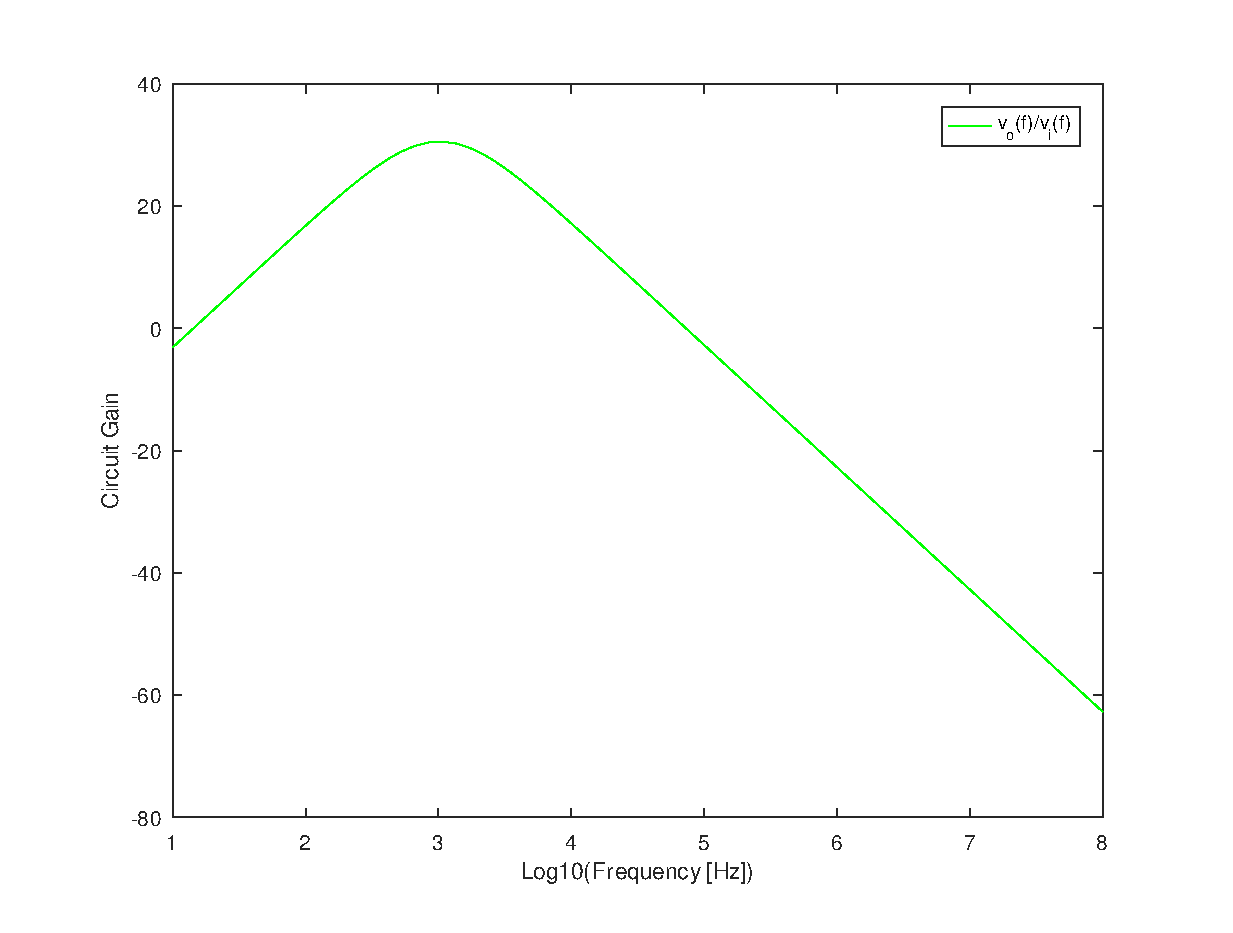
\includegraphics[width=.9\linewidth]{teoria.eps}
  \caption{Output Voltage - Theoretical Model}
  \label{fig:sim4}
\end{subfigure}
\begin{subfigure}{.5\textwidth}
  \centering
  \includegraphics[width=.9\linewidth]{vo2f.pdf}
  \caption{Output voltage - Ngspice model}
  \label{fig:sim5}
\end{subfigure}
\end{figure}

\par As we can see the graphics are pretty similar, which means that our theoretical model is a good approximation to the real running of an audio amplifier. Furthermore we can compare the values which we are studying and trying to improve: maximum gain and bandwidth and also a comparison between the operating point values is going to be made. The values are shown in the table below.

\begin{table}[H]
\parbox{.45\linewidth}{
  \centering
  \begin{tabular}{|l|r|}
    \hline    
    {\bf Calculus} & {\bf Value [V]} \\ \hline
    @gb[i] & -2.72859e-04\\ \hline
@id[current] & 1.035361e-03\\ \hline
@r1[i] & 2.604926e-04\\ \hline
@r2[i] & -2.72859e-04\\ \hline
@r3[i] & -1.23662e-05\\ \hline
@r4[i] & 1.248639e-03\\ \hline
@r5[i] & -1.30822e-03\\ \hline
@r6[i] & 9.881466e-04\\ \hline
@r7[i] & 9.881466e-04\\ \hline
v(1) & 1.216927e+01\\ \hline
v(2) & 7.480974e+00\\ \hline
v(3) & 8.035705e+00\\ \hline
v(4) & 8.297960e+00\\ \hline
v(5) & 3.074760e+00\\ \hline
v(6) & 1.005680e+00\\ \hline
v(7) & 8.073223e+00\\ \hline
v(8) & 1.005680e+00\\ \hline

  \end{tabular}
  \caption{Operating point - DC model (V) (Ngspice)}} 
\parbox{.45\linewidth}{
 \centering
  \begin{tabular}{|l|r|}
    \hline    
    {\bf Name} & {\bf Value [V]} \\ \hline
    \input{../mat/ponto0_TAB}
  \end{tabular}
  \caption{Operating point - DC model (V) (Octave)}}
\end{table}

\par As we can see the values are close and the differences that exist may be explained because of the approximations done in the transistor models.
\newpage

